\documentclass{article}\usepackage[]{graphicx}\usepackage[]{color}
%% maxwidth is the original width if it is less than linewidth
%% otherwise use linewidth (to make sure the graphics do not exceed the margin)
\makeatletter
\def\maxwidth{ %
  \ifdim\Gin@nat@width>\linewidth
    \linewidth
  \else
    \Gin@nat@width
  \fi
}
\makeatother

\definecolor{fgcolor}{rgb}{0.345, 0.345, 0.345}
\newcommand{\hlnum}[1]{\textcolor[rgb]{0.686,0.059,0.569}{#1}}%
\newcommand{\hlstr}[1]{\textcolor[rgb]{0.192,0.494,0.8}{#1}}%
\newcommand{\hlcom}[1]{\textcolor[rgb]{0.678,0.584,0.686}{\textit{#1}}}%
\newcommand{\hlopt}[1]{\textcolor[rgb]{0,0,0}{#1}}%
\newcommand{\hlstd}[1]{\textcolor[rgb]{0.345,0.345,0.345}{#1}}%
\newcommand{\hlkwa}[1]{\textcolor[rgb]{0.161,0.373,0.58}{\textbf{#1}}}%
\newcommand{\hlkwb}[1]{\textcolor[rgb]{0.69,0.353,0.396}{#1}}%
\newcommand{\hlkwc}[1]{\textcolor[rgb]{0.333,0.667,0.333}{#1}}%
\newcommand{\hlkwd}[1]{\textcolor[rgb]{0.737,0.353,0.396}{\textbf{#1}}}%
\let\hlipl\hlkwb

\usepackage{framed}
\makeatletter
\newenvironment{kframe}{%
 \def\at@end@of@kframe{}%
 \ifinner\ifhmode%
  \def\at@end@of@kframe{\end{minipage}}%
  \begin{minipage}{\columnwidth}%
 \fi\fi%
 \def\FrameCommand##1{\hskip\@totalleftmargin \hskip-\fboxsep
 \colorbox{shadecolor}{##1}\hskip-\fboxsep
     % There is no \\@totalrightmargin, so:
     \hskip-\linewidth \hskip-\@totalleftmargin \hskip\columnwidth}%
 \MakeFramed {\advance\hsize-\width
   \@totalleftmargin\z@ \linewidth\hsize
   \@setminipage}}%
 {\par\unskip\endMakeFramed%
 \at@end@of@kframe}
\makeatother

\definecolor{shadecolor}{rgb}{.97, .97, .97}
\definecolor{messagecolor}{rgb}{0, 0, 0}
\definecolor{warningcolor}{rgb}{1, 0, 1}
\definecolor{errorcolor}{rgb}{1, 0, 0}
\newenvironment{knitrout}{}{} % an empty environment to be redefined in TeX

\usepackage{alltt}
\usepackage[utf8]{inputenc}
\usepackage{hyperref}
\hypersetup{
    linktocpage,
    colorlinks=true, 
    linkcolor=blue,
    citecolor=blue,
    filecolor=blue,
    urlcolor=blue
}
\IfFileExists{upquote.sty}{\usepackage{upquote}}{}
\begin{document}

\title{Transcription vs Metilation}
\author{Lucas Michel Todó}
\maketitle
\tableofcontents
\clearpage

\begin{knitrout}
\definecolor{shadecolor}{rgb}{0.969, 0.969, 0.969}\color{fgcolor}\begin{kframe}
\begin{alltt}
\hlkwd{library}\hlstd{(ggplot2)}
\hlkwd{library}\hlstd{(reshape2)}
\end{alltt}
\end{kframe}
\end{knitrout}



\section{Taules Resum}
\subsection{Regió 5'}
\begin{knitrout}
\definecolor{shadecolor}{rgb}{0.969, 0.969, 0.969}\color{fgcolor}\begin{kframe}
\begin{verbatim}
## [1] "10G"
##    Min. 1st Qu.  Median    Mean 3rd Qu.    Max. 
##   11.28   30.53   42.98   40.40   51.08   73.44 
## [1] "1.2B"
##    Min. 1st Qu.  Median    Mean 3rd Qu.    Max. 
##   10.52   29.59   41.77   40.41   48.67   77.90 
## [1] "A7"
##    Min. 1st Qu.  Median    Mean 3rd Qu.    Max. 
##    5.56   21.81   30.12   29.55   38.11   58.04 
## [1] "C2"
##    Min. 1st Qu.  Median    Mean 3rd Qu.    Max. 
##   4.581  12.389  16.740  16.872  21.238  31.232 
## [1] "E5"
##    Min. 1st Qu.  Median    Mean 3rd Qu.    Max. 
##    5.08   17.66   24.89   24.97   33.15   51.76
\end{verbatim}
\end{kframe}
\end{knitrout}
\subsection{ORF}
\begin{knitrout}
\definecolor{shadecolor}{rgb}{0.969, 0.969, 0.969}\color{fgcolor}\begin{kframe}
\begin{verbatim}
##    Min. 1st Qu.  Median    Mean 3rd Qu.    Max. 
##   10.31   66.11   79.51   78.46   92.62  132.52 
##    Min. 1st Qu.  Median    Mean 3rd Qu.    Max. 
##   11.60   67.29   80.06   78.89   92.90  127.29 
##    Min. 1st Qu.  Median    Mean 3rd Qu.    Max. 
##   10.13   49.79   61.61   59.44   71.20   93.74 
##    Min. 1st Qu.  Median    Mean 3rd Qu.    Max. 
##   4.831  32.648  38.811  46.081  53.802 114.518 
##    Min. 1st Qu.  Median    Mean 3rd Qu.    Max. 
##   8.573  39.413  55.289  51.499  63.227  91.169
\end{verbatim}
\end{kframe}
\end{knitrout}
\subsection{Regió 3'}
\begin{knitrout}
\definecolor{shadecolor}{rgb}{0.969, 0.969, 0.969}\color{fgcolor}\begin{kframe}
\begin{verbatim}
##    Min. 1st Qu.  Median    Mean 3rd Qu.    Max. 
##   2.891   7.493  10.409  11.215  12.818  40.575 
##    Min. 1st Qu.  Median    Mean 3rd Qu.    Max. 
##   4.807  11.271  15.083  15.651  18.253  42.265 
##    Min. 1st Qu.  Median    Mean 3rd Qu.    Max. 
##   2.994   5.297   7.814   7.895   9.344  22.439 
##    Min. 1st Qu.  Median    Mean 3rd Qu.    Max. 
##   2.165   4.060   5.580   5.707   6.934  17.490 
##    Min. 1st Qu.  Median    Mean 3rd Qu.    Max. 
##  0.7938  1.5479  2.4806  2.9586  4.0980  9.4463
\end{verbatim}
\end{kframe}
\end{knitrout}
\clearpage


\section{Gràfics}
\subsection{Coverage}
\begin{knitrout}
\definecolor{shadecolor}{rgb}{0.969, 0.969, 0.969}\color{fgcolor}
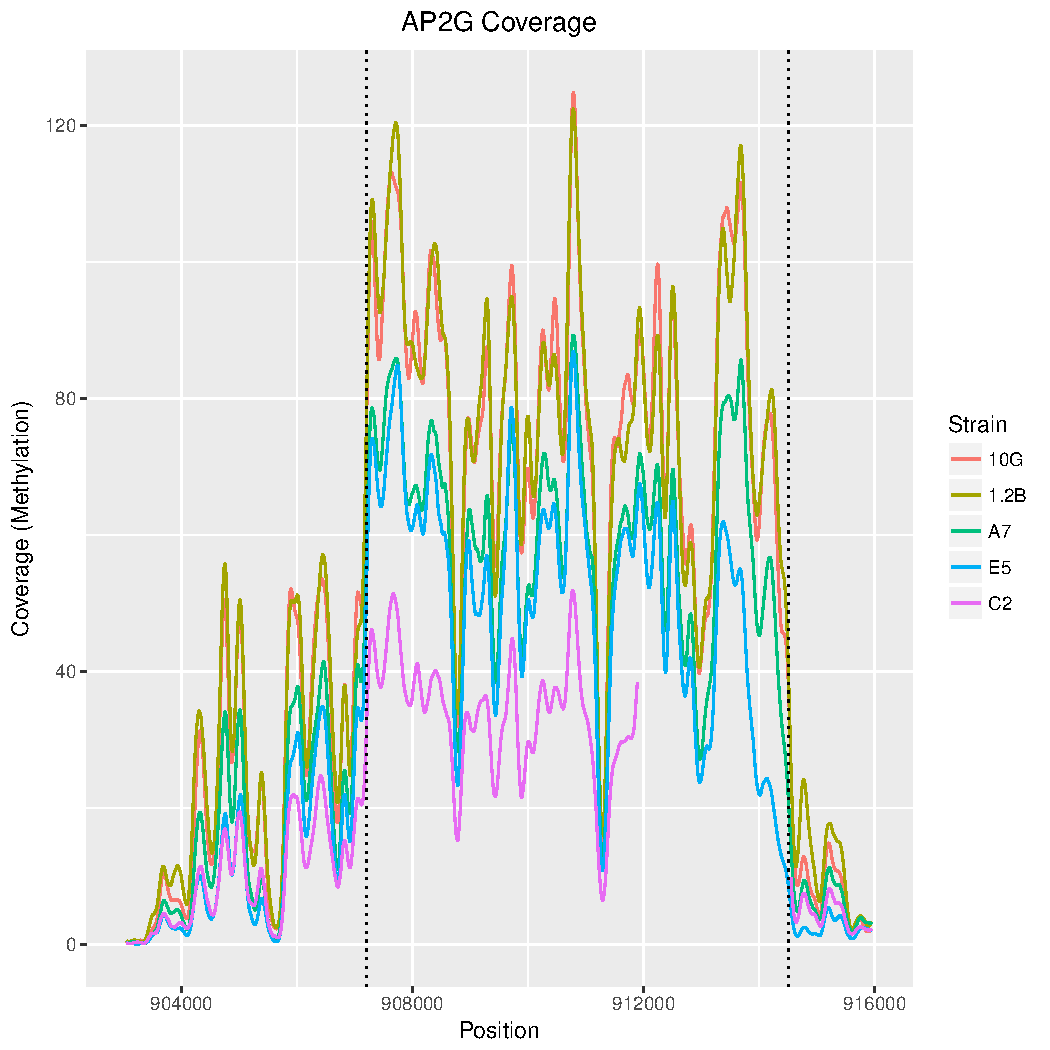
\includegraphics[width=1\linewidth]{figure/plot_coverage-1} 

\end{knitrout}
\clearpage
\subsection{Coverage Normalitzat}
\begin{knitrout}
\definecolor{shadecolor}{rgb}{0.969, 0.969, 0.969}\color{fgcolor}
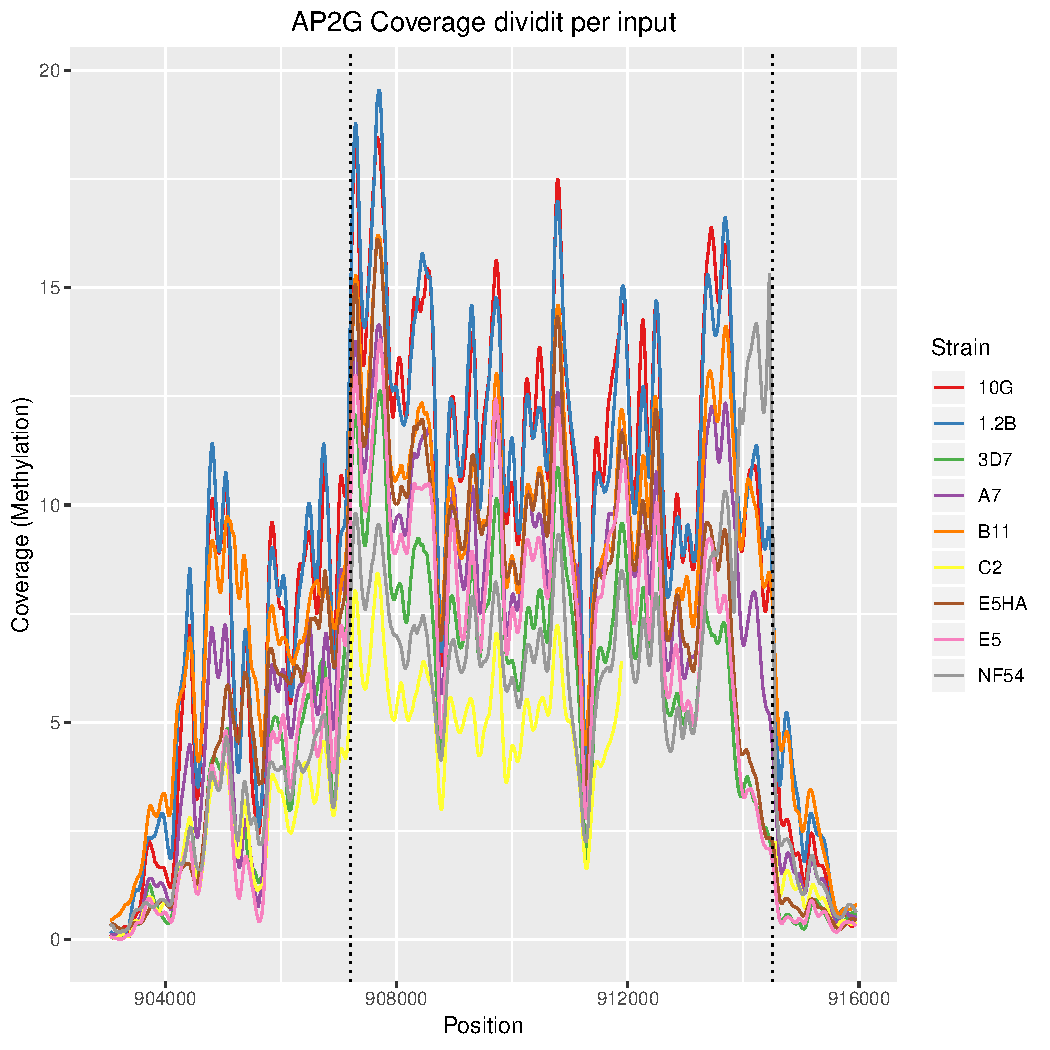
\includegraphics[width=1\linewidth]{figure/plot_norm_cov-1} 

\end{knitrout}
\clearpage
\subsection{Coverage Normalitzat a regió 5'}
\begin{knitrout}
\definecolor{shadecolor}{rgb}{0.969, 0.969, 0.969}\color{fgcolor}
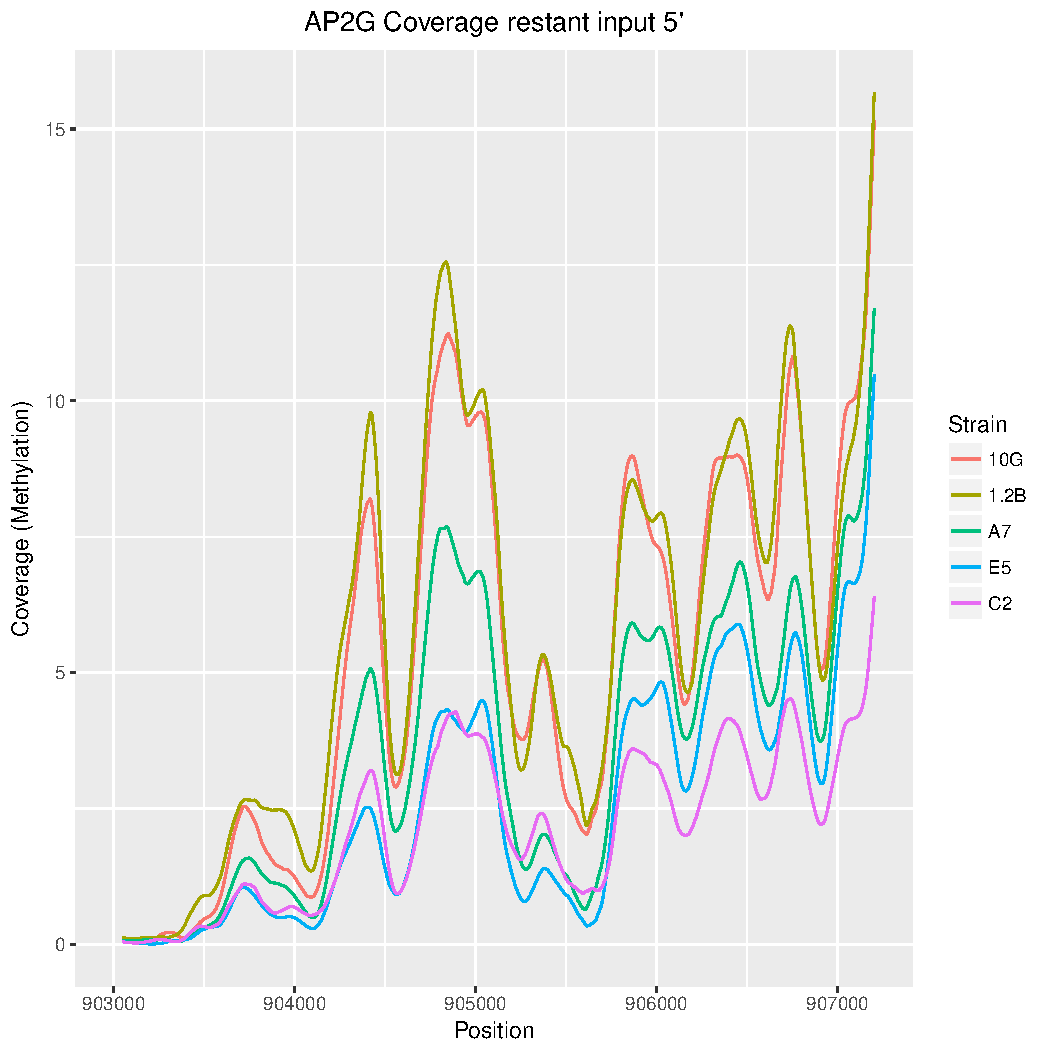
\includegraphics[width=1\linewidth]{figure/plot_norm_cov_5-1} 

\end{knitrout}
\clearpage
\subsection{Coverage Acetilació}
\begin{knitrout}
\definecolor{shadecolor}{rgb}{0.969, 0.969, 0.969}\color{fgcolor}
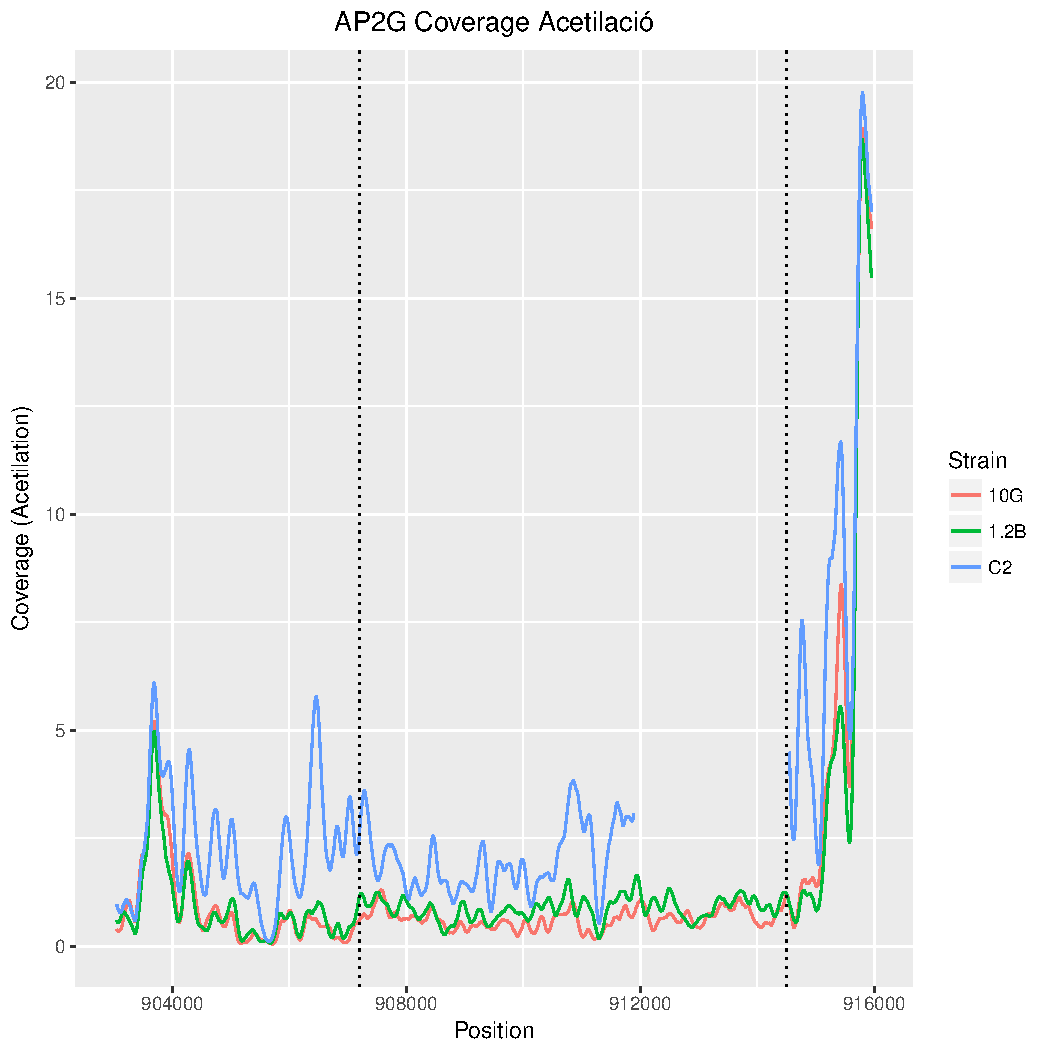
\includegraphics[width=1\linewidth]{figure/plot_ac-1} 

\end{knitrout}
\clearpage
\subsection{Coverage Acetilació a 5'}
\begin{knitrout}
\definecolor{shadecolor}{rgb}{0.969, 0.969, 0.969}\color{fgcolor}
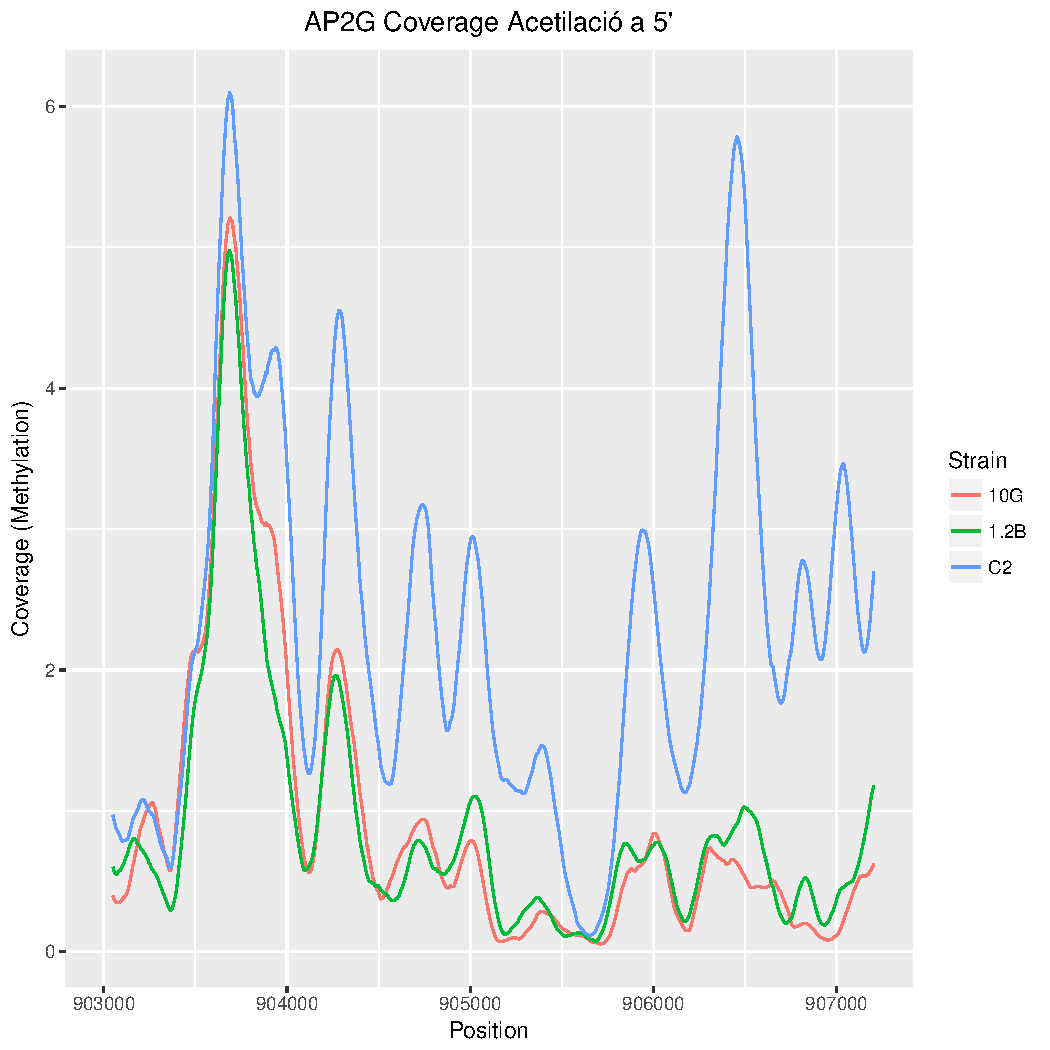
\includegraphics[width=1\linewidth]{figure/plot_ac_5-1} 

\end{knitrout}
\clearpage

\begin{knitrout}
\definecolor{shadecolor}{rgb}{0.969, 0.969, 0.969}\color{fgcolor}\begin{kframe}
\begin{alltt}
\hlstd{df_ac_met} \hlkwb{<-} \hlstd{df_ac[,}\hlopt{-}\hlnum{4}\hlstd{]} \hlopt{/} \hlstd{df[,}\hlkwd{c}\hlstd{(}\hlnum{1}\hlstd{,}\hlnum{2}\hlstd{,}\hlnum{5}\hlstd{)]}
\hlstd{df_ac_met[}\hlstr{"pos"}\hlstd{]} \hlkwb{<-} \hlstd{df}\hlopt{$}\hlstd{pos}
\hlstd{df_ac_met_m} \hlkwb{<-} \hlkwd{melt}\hlstd{(df_ac_met,} \hlkwc{id} \hlstd{=} \hlstr{"pos"}\hlstd{)}

\hlstd{p} \hlkwb{<-} \hlkwd{ggplot}\hlstd{(df_ac_met_m,} \hlkwd{aes}\hlstd{(}\hlkwc{x} \hlstd{= pos,} \hlkwc{y} \hlstd{= df_ac_met_m}\hlopt{$}\hlstd{value,} \hlkwc{colour} \hlstd{= df_ac_met_m}\hlopt{$}\hlstd{variable))}
\hlstd{p} \hlopt{+} \hlkwd{geom_line}\hlstd{()} \hlopt{+}
    \hlkwd{labs}\hlstd{(}\hlkwc{title} \hlstd{=} \hlstr{"AP2G Coverage Acetilació"}\hlstd{,} \hlkwc{x} \hlstd{=} \hlstr{"Position"}\hlstd{,} \hlkwc{y} \hlstd{=} \hlstr{"Coverage (Methylation)"}\hlstd{,} \hlkwc{colour} \hlstd{=} \hlstr{"Strain"}\hlstd{)} \hlopt{+}
    \hlkwd{theme}\hlstd{(}\hlkwc{plot.title} \hlstd{=} \hlkwd{element_text}\hlstd{(}\hlkwc{hjust} \hlstd{=} \hlnum{0.5}\hlstd{))}
\end{alltt}
\end{kframe}
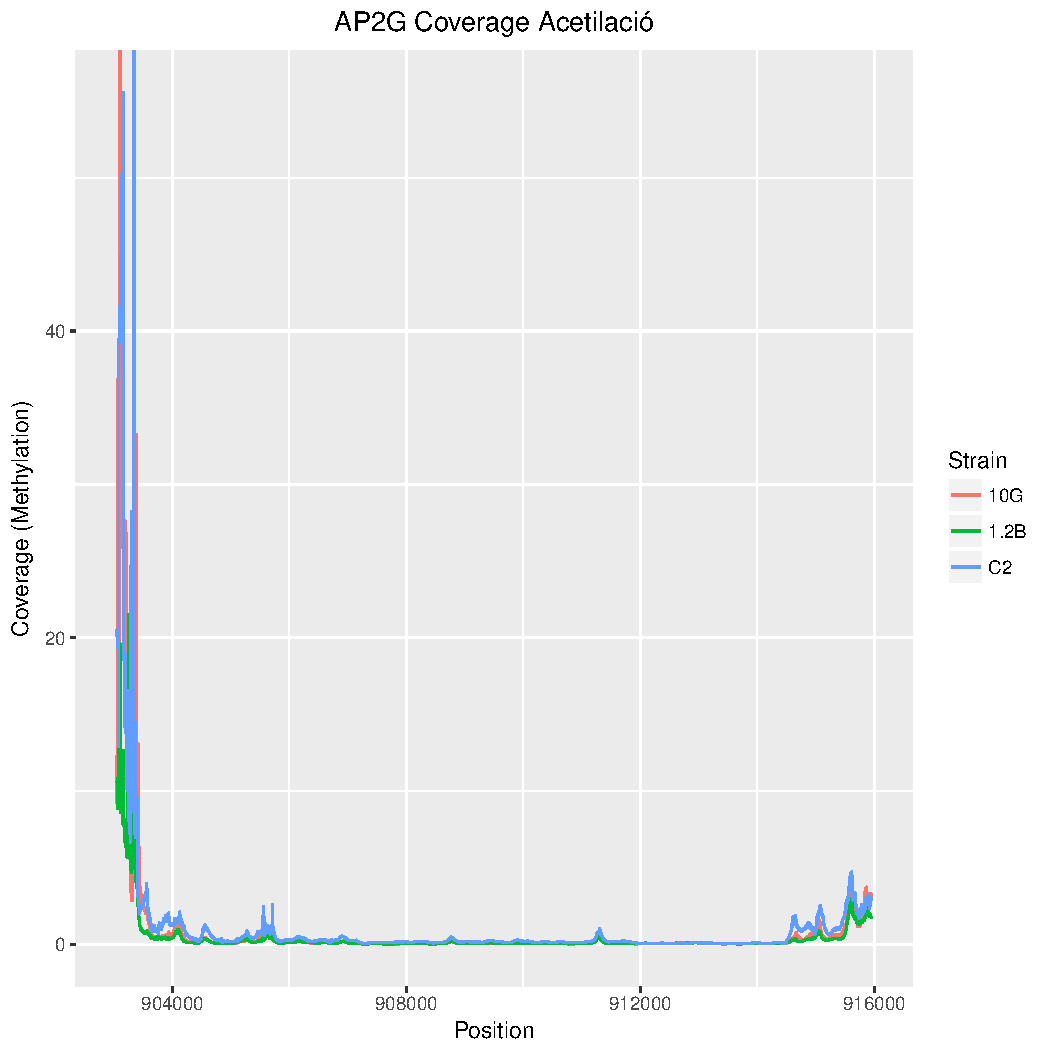
\includegraphics[width=\maxwidth]{figure/unnamed-chunk-1-1} 

\end{knitrout}
\end{document}
